\documentclass[aspectratio=169,12pt]{beamer}
\usepackage[utf8]{inputenc}
\usepackage{amsmath, amssymb}
\usepackage{array}
\usepackage{booktabs}
\usepackage{colortbl}
\usepackage{hyperref}
\usepackage{makecell}
\usepackage{ragged2e}
\usepackage{bytefield}
\usepackage{tikz}
\usetikzlibrary{arrows.meta, positioning, shapes.geometric, calc, tikzmark, shapes.misc, automata, backgrounds, matrix}
\usepackage{tcolorbox}

% Define colors
\definecolor{myblue}{RGB}{0,0,255}
\definecolor{mypurple}{RGB}{128,0,128}
\definecolor{mygreen}{RGB}{0,128,0}
\definecolor{myorange}{RGB}{255,140,0}
\definecolor{lightblue}{RGB}{173,216,230}
\definecolor{peach}{RGB}{255,218,185}
\definecolor{lightpurple}{RGB}{230,230,250}

\usetheme{Madrid}
\setbeamertemplate{navigation symbols}{}

\title{Branch Prediction}
\author{Computer Architecture 2340267}
\date{2025, Lecture \#6}

\begin{document}

\frame{\titlepage}

\begin{frame}{Outline}
\tableofcontents
\end{frame}

% The Branch Prediction Unit in the Pipeline
\begin{frame}
\frametitle{The Branch Prediction Unit in the Pipeline}
\label{frame:bpu_pipeline}

% TODO: Add pipeline diagram showing BPU integration
% See PDF page 2 for reference diagram
\begin{center}
\textcolor{red}{[PLACEHOLDER: Pipeline diagram with BPU, showing Fetch/Decode/Execute/Memory/WB stages]}
\end{center}

\vspace{0.3cm}

\begin{itemize}
    \item \textbf{Lookup BPU in parallel to I\$}
    \begin{itemize}
        \item BPU provides the predicted target and direction at fetch
    \end{itemize}
\end{itemize}

\vspace{0.2cm}

\begin{itemize}
    \item \textbf{At Execute stage}
    \begin{itemize}
        \item Verify direction (T/NT) and target (if taken)
        \item Flush if mis-predict
        \item Update/allocate BPU
    \end{itemize}
\end{itemize}

\end{frame}

% Section title - Branches and Performance
\begin{frame}
\frametitle{Branches and Performance}
\label{frame:branches_performance}

\begin{itemize}
    \item \textbf{Misprediction Rate (MPR) vs. Misprediction Per Instruction (MPI)}
\end{itemize}

\vspace{0.3cm}

\begin{center}
\begin{tabular}{ccc}
$\text{MPR} = \dfrac{\text{\# mis-predicted jumps}}{\text{total \# jump}}$ & \hspace{1cm} & $\text{MPI} = \dfrac{\text{\# mis-predicted jumps}}{\text{total \# instructions}}$
\end{tabular}
\end{center}

\vspace{0.3cm}

\begin{itemize}
    \item MPI correlates better with performance since it takes into account jumps frequency
\end{itemize}

\vspace{0.2cm}

\begin{itemize}
    \item \textbf{Assume}
    \begin{itemize}
        \item MPI = 1\% (1 flush every 100 instructions on average)
        \item IPC=2 \hspace{0.5cm} (2 instructions per cycle on average)
        \item Flush penalty of 10 cycles
    \end{itemize}
\end{itemize}

\vspace{0.2cm}

\begin{itemize}
    \item \textbf{We get:}
    \begin{itemize}
        \item MPI = 1\% $\Rightarrow$ 1 flush every 100 instructions on average
        \item IPC=2 $\Rightarrow$ 1 flush every 50 cycles
        \item 10 cycles flush penalty every 50 cycles
        \item 20\% in performance
    \end{itemize}
\end{itemize}

\end{frame}

\begin{frame}
\frametitle{What/Who/When We Predict/Fix/Allocate}
\label{frame:predict_fix_allocate}

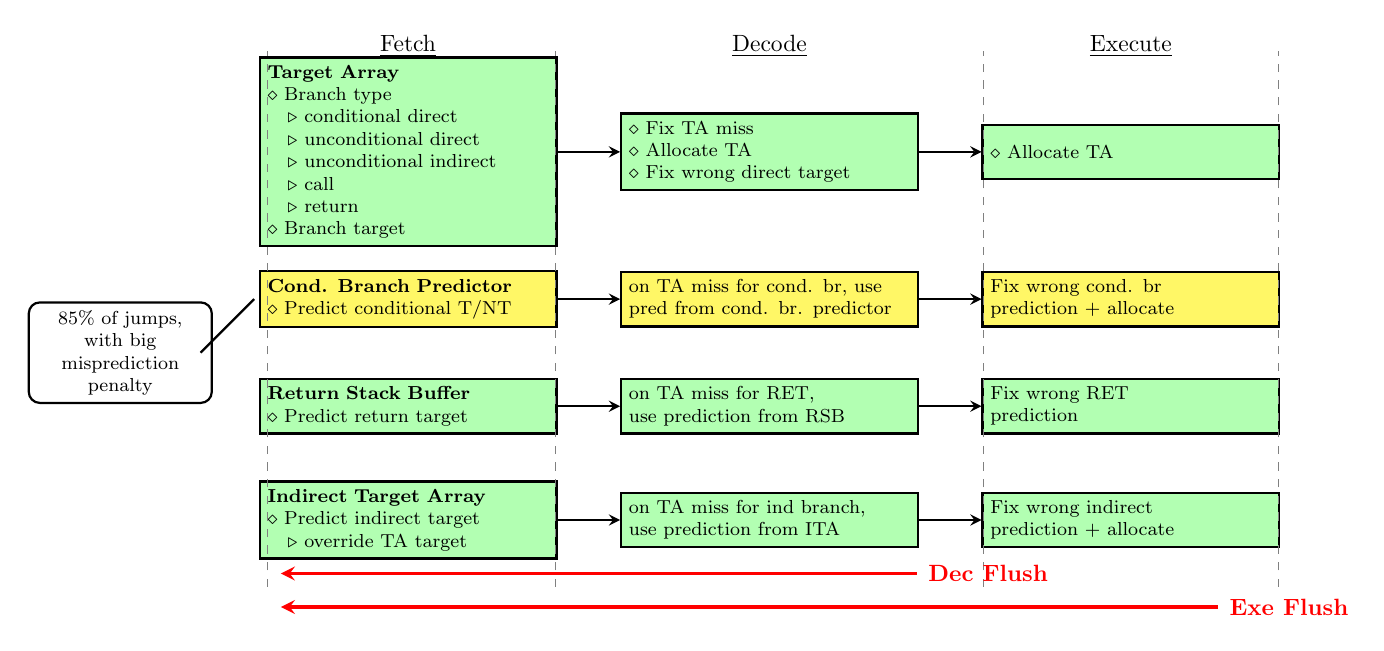
\begin{tikzpicture}[scale=0.85, transform shape,
    box/.style={rectangle, draw=black, thick, minimum height=0.8cm, text width=4.2cm, align=left, font=\footnotesize},
    greenbox/.style={box, fill=green!30},
    yellowbox/.style={box, fill=yellow!60},
    arrow/.style={->, thick, >=stealth}
]

% Column headers
\node[font=\normalsize, anchor=south] at (2.1, 5.8) {\underline{Fetch}};
\node[font=\normalsize, anchor=south] at (7.5, 5.8) {\underline{Decode}};
\node[font=\normalsize, anchor=south] at (12.9, 5.8) {\underline{Execute}};

% Fetch column
\node[greenbox] (ta) at (2.1, 4.5) {
    \textbf{Target Array}\\
    $\diamond$ Branch type\\
    \hspace{0.3cm}$\triangleright$ conditional direct\\
    \hspace{0.3cm}$\triangleright$ unconditional direct\\
    \hspace{0.3cm}$\triangleright$ unconditional indirect\\
    \hspace{0.3cm}$\triangleright$ call\\
    \hspace{0.3cm}$\triangleright$ return\\
    $\diamond$ Branch target
};

\node[yellowbox] (cbp) at (2.1, 2.3) {
    \textbf{Cond. Branch Predictor}\\
    $\diamond$ Predict conditional T/NT
};

\node[greenbox] (rsb) at (2.1, 0.7) {
    \textbf{Return Stack Buffer}\\
    $\diamond$ Predict return target
};

\node[greenbox] (ita) at (2.1, -1.0) {
    \textbf{Indirect Target Array}\\
    $\diamond$ Predict indirect target\\
    \hspace{0.3cm}$\triangleright$ override TA target
};

% Decode column
\node[greenbox] (dec1) at (7.5, 4.5) {
    $\diamond$ Fix TA miss\\
    $\diamond$ Allocate TA\\
    $\diamond$ Fix wrong direct target
};

\node[yellowbox] (dec2) at (7.5, 2.3) {
    on TA miss for cond. br, use\\
    pred from cond. br. predictor
};

\node[greenbox] (dec3) at (7.5, 0.7) {
    on TA miss for RET,\\
    use prediction from RSB
};

\node[greenbox] (dec4) at (7.5, -1.0) {
    on TA miss for ind branch,\\
    use prediction from ITA
};

% Execute column
\node[greenbox] (exe1) at (12.9, 4.5) {
    $\diamond$ Allocate TA
};

\node[yellowbox] (exe2) at (12.9, 2.3) {
    Fix wrong cond. br\\
    prediction + allocate
};

\node[greenbox] (exe3) at (12.9, 0.7) {
    Fix wrong RET\\
    prediction
};

\node[greenbox] (exe4) at (12.9, -1.0) {
    Fix wrong indirect\\
    prediction + allocate
};

% Arrows between columns
\draw[arrow] (ta.east) -- (dec1.west);
\draw[arrow] (cbp.east) -- (dec2.west);
\draw[arrow] (rsb.east) -- (dec3.west);
\draw[arrow] (ita.east) -- (dec4.west);

\draw[arrow] (dec1.east) -- (exe1.west);
\draw[arrow] (dec2.east) -- (exe2.west);
\draw[arrow] (dec3.east) -- (exe3.west);
\draw[arrow] (dec4.east) -- (exe4.west);

% Vertical dashed lines
\draw[dashed, gray] (0, -2) -- (0, 6);
\draw[dashed, gray] (4.3, -2) -- (4.3, 6);
\draw[dashed, gray] (10.7, -2) -- (10.7, 6);
\draw[dashed, gray] (15.1, -2) -- (15.1, 6);

% Left annotation
\node[draw, rounded corners, thick, text width=2.5cm, align=center, font=\footnotesize] at (-2.2, 1.5) {
    85\% of jumps,\\
    with big\\
    misprediction\\
    penalty
};
\draw[thick] (-1.0, 1.5) -- (-0.2, 2.3);


% Red flush arrows (arrow ends just before the text)
\draw[arrow, red, very thick] (9.7, -1.8) -- (0.2, -1.8);
\node[red, font=\normalsize, anchor=west] at (9.75, -1.8) {\textbf{Dec Flush}};

\draw[arrow, red, very thick] (14.2, -2.3) -- (0.2, -2.3);
\node[red, font=\normalsize, anchor=west] at (14.25, -2.3) {\textbf{Exe Flush}};

\end{tikzpicture}

\end{frame}

% Third Slide - The Target Array
\begin{frame}
\frametitle{The Target Array}
\label{frame:target_array}

\begin{columns}[T]
\begin{column}{0.58\textwidth}
\begin{itemize}
    \item \textbf{The TA is accessed using the branch address (branch IP)}
    \begin{itemize}
        \item Implemented as an $n$-way set associative cache
    \end{itemize}
\end{itemize}

\vspace{0.15cm}

\begin{itemize}
    \item \textbf{The TA predicts the following}
    \begin{itemize}
        \item Instruction is a branch
        \item Predicted target
        \item Branch type
        \begin{itemize}
            \item Conditional: jump to target if predict taken
            \item Unconditional direct: take target
            \item Unconditional Indirect: if ITA hits, use its target
            \item Return: get target from Return Stack Buffer
        \end{itemize}
    \end{itemize}
\end{itemize}

\vspace{0.15cm}

\begin{itemize}
    \item \textbf{The TA is allocated/updated at Decode / EXE}
\end{itemize}

\vspace{0.15cm}

\begin{itemize}
    \item \textbf{Tags are usually partial}
    \begin{itemize}
        \item Trade-off space, can get false hits
        \item Few branches aliased to same entry
        \item No \textit{correctness}, only \textit{performance}
    \end{itemize}
\end{itemize}
\end{column}

\begin{column}{0.42\textwidth}
\vspace{0.5cm}
\begin{center}
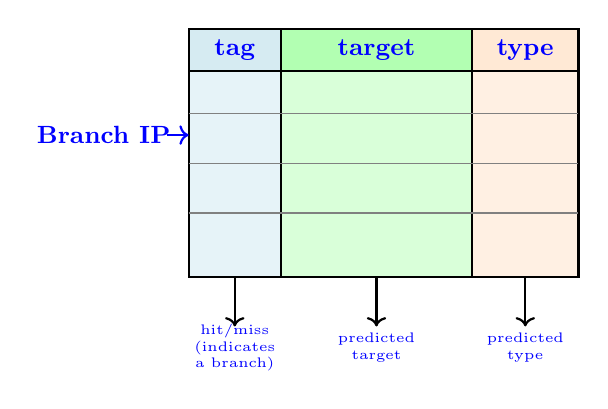
\begin{tikzpicture}[scale=0.9]
    % Define dimensions
    \def\tablewidth{5.5}
    \def\tableheight{3.5}
    \def\headerheight{0.6}
    \def\tagwidth{1.3}
    \def\targetwidth{2.7}
    \def\typewidth{1.5}
    
    % Draw the main table structure with colored columns
    % Tag column background
    \fill[lightblue!30] (0,0) rectangle (\tagwidth, -\tableheight);
    % Target column background  
    \fill[green!15] (\tagwidth,0) rectangle (\tagwidth+\targetwidth, -\tableheight);
    % Type column background
    \fill[peach!40] (\tagwidth+\targetwidth,0) rectangle (\tablewidth, -\tableheight);
    
    % Draw header row with stronger colors
    \fill[lightblue!50] (0,0) rectangle (\tagwidth, -\headerheight);
    \fill[green!30] (\tagwidth,0) rectangle (\tagwidth+\targetwidth, -\headerheight);
    \fill[peach!60] (\tagwidth+\targetwidth,0) rectangle (\tablewidth, -\headerheight);
    
    % Draw the table border
    \draw[thick, black] (0,0) rectangle (\tablewidth, -\tableheight);
    
    % Draw column dividers
    \draw[thick] (\tagwidth, 0) -- (\tagwidth, -\tableheight);
    \draw[thick] (\tagwidth+\targetwidth, 0) -- (\tagwidth+\targetwidth, -\tableheight);
    
    % Draw header separator
    \draw[thick] (0, -\headerheight) -- (\tablewidth, -\headerheight);
    
    % Add some row lines to show it's a table
    \foreach \y in {1.2, 1.9, 2.6} {
        \draw[gray, thin] (0, -\y) -- (\tablewidth, -\y);
    }
    
    % Header labels
    \node[myblue, font=\small\bfseries] at (\tagwidth/2, -\headerheight/2) {tag};
    \node[myblue, font=\small\bfseries] at (\tagwidth+\targetwidth/2, -\headerheight/2) {target};
    \node[myblue, font=\small\bfseries] at (\tagwidth+\targetwidth+\typewidth/2, -\headerheight/2) {type};
    
    % Branch IP label and arrow pointing to table
    \node[myblue, font=\small\bfseries] at (-1.2, -1.5) {Branch IP};
    \draw[->, thick, myblue] (-0.3, -1.5) -- (0, -1.5);
    
    % Output arrows and labels below the table
    \draw[->, thick] (\tagwidth/2, -\tableheight) -- (\tagwidth/2, -\tableheight-0.7);
    \node[align=center, font=\tiny, myblue] at (\tagwidth/2, -\tableheight-1.0) {hit/miss\\(indicates\\a branch)};
    
    \draw[->, thick] (\tagwidth+\targetwidth/2, -\tableheight) -- (\tagwidth+\targetwidth/2, -\tableheight-0.7);
    \node[align=center, font=\tiny, myblue] at (\tagwidth+\targetwidth/2, -\tableheight-1.0) {predicted\\target};
    
    \draw[->, thick] (\tagwidth+\targetwidth+\typewidth/2, -\tableheight) -- (\tagwidth+\targetwidth+\typewidth/2, -\tableheight-0.7);
    \node[align=center, font=\tiny, myblue] at (\tagwidth+\targetwidth+\typewidth/2, -\tableheight-1.0) {predicted\\type};
\end{tikzpicture}
\end{center}
\end{column}
\end{columns}

\end{frame}




\begin{frame}{The Target Array}
\begin{columns}[T,onlytextwidth]
  \begin{column}{0.63\textwidth}
    \begin{itemize}
      \item The TA is accessed using the branch address (branch IP)
      \begin{itemize}
        \item Implemented as an $n$-way set associative cache
      \end{itemize}

      \item The TA predicts the following
      \begin{itemize}
        \item Instruction is a branch
        \item Predicted target
        \item Branch type
        \begin{itemize}
          \item Conditional: jump to target if predict taken
          \item Unconditional direct: take target
          \item Unconditional indirect: if iTA hits, use its target
          \item Return: get target from Return Stack Buffer
        \end{itemize}
      \end{itemize}

      \item The TA is allocated/updated at Decode / EXE

      \item Tags are usually partial
      \begin{itemize}
        \item Trade-off space, can get false hits
        \item Few branches aliased to same entry
        \item No correctness, only performance
      \end{itemize}
    \end{itemize}
  \end{column}

  \begin{column}{0.37\textwidth}
    \centering
    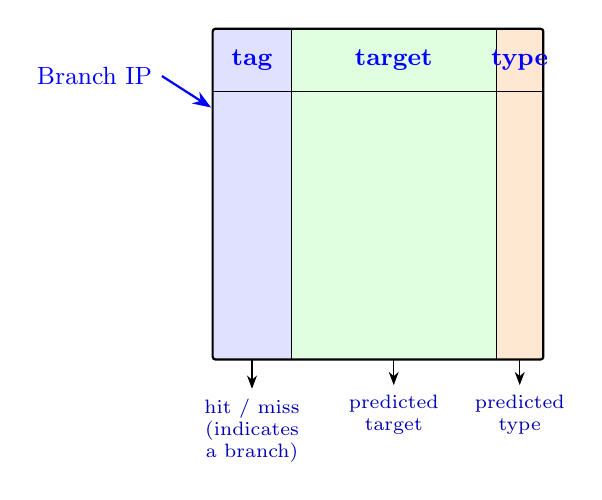
\begin{tikzpicture}[>=Stealth, node distance=2mm]
      % Sizes
      \def\W{4.2}   % total width
      \def\H{4.2}   % total height
      \def\tagw{1.0}
      \def\targetw{2.6}
      \def\typew{0.6}

      % Background column tints
      \fill[blue!12]   (0,-\H) rectangle (\tagw,0);
      \fill[green!12]  (\tagw,-\H) rectangle (\tagw+\targetw,0);
      \fill[orange!18] (\tagw+\targetw,-\H) rectangle (\W,0);

      % Outer box
      \draw[rounded corners=1pt, line width=0.8pt] (0,0) rectangle (\W,-\H);

      % Column dividers
      \draw (\tagw,0) -- (\tagw,-\H);
      \draw (\tagw+\targetw,0) -- (\tagw+\targetw,-\H);

      % Header separator
      \draw (0,-0.8) -- (\W,-0.8);

      % Header labels
      \node[font=\small\bfseries,blue]   at ($(0,0)!0.5!(\tagw,0)+(0,-0.4)$) {tag};
      \node[font=\small\bfseries,blue]   at ($(\tagw,0)!0.5!(\tagw+\targetw,0)+(0,-0.4)$) {target};
      \node[font=\small\bfseries,blue]   at ($(\tagw+\targetw,0)!0.5!(\W,0)+(0,-0.4)$) {type};

      % Branch IP input (left)
      \node[align=left, blue] (bp) at (-1.5,-0.6) {\small Branch IP};
      \draw[->,blue,thick] (bp.east) -- (-0.02,-1.0);

      % Bottom outputs
      \node[align=center, font=\scriptsize, blue!70!black] (hit) at (\tagw/2,-\H-0.9) {hit / miss\\(indicates\\a branch)};
      \draw[->] (\tagw/2,-\H) -- (hit.north);

      \node[align=center, font=\scriptsize, blue!70!black] (pt) at (\tagw+\targetw/2,-\H-0.7) {predicted\\target};
      \draw[->] (\tagw+\targetw/2,-\H) -- (pt.north);

      \node[align=center, font=\scriptsize, blue!70!black] (ty) at (\tagw+\targetw+\typew/2,-\H-0.7) {predicted\\type};
      \draw[->] (\tagw+\targetw+\typew/2,-\H) -- (ty.north);
    \end{tikzpicture}
  \end{column}
\end{columns}
\end{frame}


% Second Slide (previously first)
\begin{frame}
\frametitle{Bimodal Predictor (cont.)}
\label{frame:bimodal_predictor_cont}

\vspace{-0.2cm}

\begin{center}
\textcolor{myblue}{\textbf{2-bit-sat counter array}}
\end{center}

\vspace{0.2cm}

\begin{center}
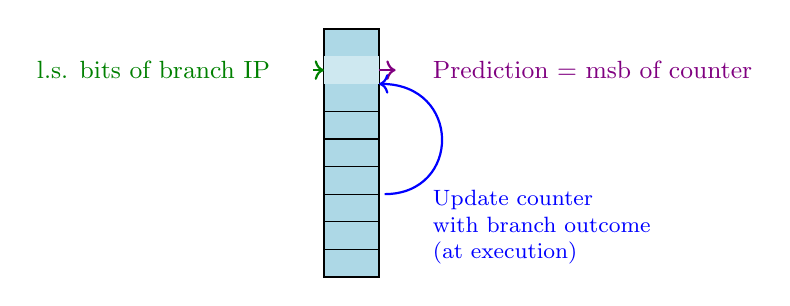
\begin{tikzpicture}[scale=0.7]
    % Draw the counter array
    \fill[lightblue] (0,0) rectangle (1,4.5);
    \draw[thick] (0,0) rectangle (1,4.5);
    
    % Draw array divisions
    \foreach \y in {0.5,1,1.5,2,2.5,3,3.5,4} {
        \draw (0,\y) -- (1,\y);
    }
    
    % Highlight the second cell from top (the one being accessed)
    \fill[lightblue!60] (0,3.5) rectangle (1,4);
    
    % Labels and arrows - pointing to second cell from top
    \node[mygreen,anchor=east,font=\small] at (-0.8,3.75) {l.s. bits of branch IP};
    \draw[->,thick,mygreen] (-0.2,3.75) -- (0,3.75);
    
    \node[mypurple,anchor=west,font=\small] at (1.8,3.75) {Prediction = msb of counter};
    \draw[->,thick,mypurple] (1,3.75) -- (1.3,3.75);
    
    % Curved arrow for update - starting low and curving up to second cell
    \draw[->,thick,myblue] (1.1,1.5) .. controls (2.5,1.5) and (2.5,3.5) .. (1,3.5);
    \node[myblue,align=left,anchor=west,font=\footnotesize] at (1.8,0.9) {Update counter\\with branch outcome\\(at execution)};
\end{tikzpicture}
\end{center}

\vspace{0.3cm}

\begin{itemize}
    \item \small\textbf{2-bit predictor avoids a double mistake in loops / glitches from the pattern}
\end{itemize}

\vspace{0.1cm}

{\footnotesize
\begin{tabular}{@{}ll@{}}
Branch Outcome & \texttt{0 0 0 0 0 1 0 0 0 0 0 1 0 0 0 0 0 1} \\
Prediction & \texttt{?~0 0 0 0 \textcolor{red}{0} 0 0 0 0 0 \textcolor{red}{0} 0 0 0 0 0 0} \\
\end{tabular}
}

\end{frame}


% Third Slide (previously second)
\begin{frame}
\frametitle{Bimodal (2-bit) Predictor}
\label{frame:bimodal_2bit}

%\vspace{-0.3cm}

\begin{itemize}
    \item \textbf{A 2-bit counter avoids the double mistake in glitches}
    \begin{itemize}
        \item Need "more evidence" to change prediction
    \end{itemize}
\end{itemize}

\vspace{-0.2cm}

\begin{center}
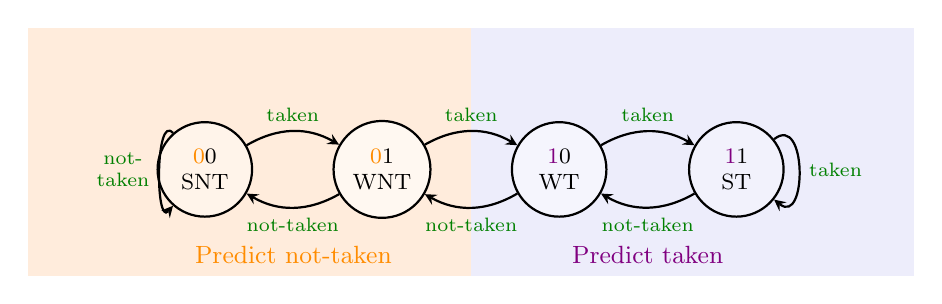
\begin{tikzpicture}[
    state/.style={circle,draw,thick,minimum size=1.2cm,font=\footnotesize,align=center},
    arrow/.style={->,>=stealth,thick},
    scale=0.9
]
    % Distinct background shades for prediction regions
    \begin{scope}[on background layer]
        \fill[peach!50] (-2.5,-1.5) rectangle (3.75,2); % Predict not-taken region
        \fill[lightpurple!70] (3.75,-1.5) rectangle (10,2); % Predict taken region, extended further right
    \end{scope}
    
    % States (LSB in black)
    \node[state,fill=peach!30] (SNT) at (0,0) {\textcolor{myorange}{0}\textcolor{black}{0}\\SNT};
    \node[state,fill=peach!20] (WNT) at (2.5,0) {\textcolor{myorange}{0}\textcolor{black}{1}\\WNT};
    \node[state,fill=lightpurple!40] (WT) at (5,0) {\textcolor{mypurple}{1}\textcolor{black}{0}\\WT};
    \node[state,fill=lightpurple!50] (ST) at (7.5,0) {\textcolor{mypurple}{1}\textcolor{black}{1}\\ST};
    
    % Self loop for SNT: from top left to bottom left, label on two lines
    \draw[arrow] (SNT) .. controls (-0.7,0.8) and (-0.7,-0.8) .. node[left,mygreen,font=\scriptsize,align=center] {not-\\taken} (SNT);
    % Self loop for ST: from top right to bottom right
    \draw[arrow] (ST) .. controls (8.5,0.8) and (8.5,-0.8) .. node[right,mygreen,font=\scriptsize,align=center] {taken} (ST);
    
    % Transitions between states
    \draw[arrow] (SNT) to[bend left=30] node[above,mygreen,font=\scriptsize] {taken} (WNT);
    \draw[arrow] (WNT) to[bend left=30] node[below,mygreen,font=\scriptsize] {not-taken} (SNT);
    
    \draw[arrow] (WNT) to[bend left=30] node[above,mygreen,font=\scriptsize] {taken} (WT);
    \draw[arrow] (WT) to[bend left=30] node[below,mygreen,font=\scriptsize] {not-taken} (WNT);
    
    \draw[arrow] (WT) to[bend left=30] node[above,mygreen,font=\scriptsize] {taken} (ST);
    \draw[arrow] (ST) to[bend left=30] node[below,mygreen,font=\scriptsize] {not-taken} (WT);
    
    % Prediction labels
    \node[myorange,font=\small] at (1.25,-1.2) {Predict not-taken};
    \node[mypurple,font=\small] at (6.25,-1.2) {Predict taken};
\end{tikzpicture}
\end{center}

\vspace{0.1cm}

\begin{itemize}
    \item Initial state: weakly-taken (most branches are taken)
\end{itemize}

\begin{itemize}
    \item \textbf{Update (at execution)}
    \begin{itemize}
        \item Branch was actually taken: increment counter (saturate at 11)
        \item Branch was actually not-taken: decrement counter (saturate at 00)
    \end{itemize}
\end{itemize}

\begin{itemize}
    \item \textbf{Predict according to m.s.bit of counter (0=NT, 1=taken)}
    \item \textbf{Does not predict well branches with patterns like 010101...}
\end{itemize}

\end{frame}

\begin{frame}
\frametitle{Bimodal Predictor - example}
\label{frame:bimodal_example}

\begin{columns}[T]
\begin{column}{0.62\textwidth}

% Br1 prediction with tabular and vertical arrows
\begin{itemize}
\item \textbf{Br1 prediction}
\end{itemize}
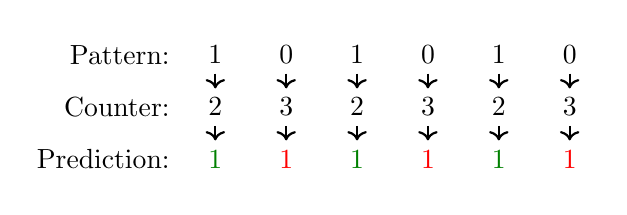
\begin{tikzpicture}[baseline=(current bounding box.center),every node/.style={anchor=base}]
    % Table for alignment
    \matrix[matrix of nodes,nodes={minimum width=0.5cm,anchor=center},column sep=0.4cm,row sep=0.2cm,ampersand replacement=\&] (m) {
        1 \& 0 \& 1 \& 0 \& 1 \& 0 \\
        2 \& 3 \& 2 \& 3 \& 2 \& 3 \\
        \textcolor{mygreen}{1} \& \textcolor{red}{1} \& \textcolor{mygreen}{1} \& \textcolor{red}{1} \& \textcolor{mygreen}{1} \& \textcolor{red}{1} \\
    };
    % Arrows from pattern to counter
    \foreach \i in {1,...,6} {
        \draw[->,thick] (m-1-\i.south) -- (m-2-\i.north);
        \draw[->,thick] (m-2-\i.south) -- (m-3-\i.north);
    }
    % Labels
    \node[left=0.2cm of m-1-1,align=right] {Pattern:};
    \node[left=0.2cm of m-2-1,align=right] {Counter:};
    \node[left=0.2cm of m-3-1,align=right] {Prediction:};
\end{tikzpicture}

\vspace{0.2cm}
% Br2 prediction with tabular and vertical arrows
\begin{itemize}
\item \textbf{Br2 prediction}
\end{itemize}
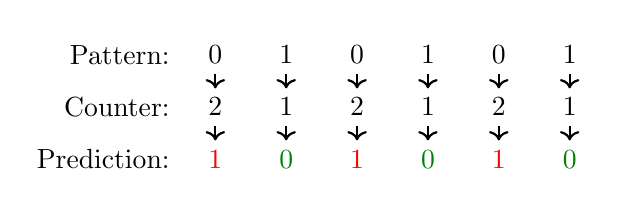
\begin{tikzpicture}[baseline=(current bounding box.center),every node/.style={anchor=base}]
    % Table for alignment
    \matrix[matrix of nodes,nodes={minimum width=0.5cm,anchor=center},column sep=0.4cm,row sep=0.2cm,ampersand replacement=\&] (m) {
        0 \& 1 \& 0 \& 1 \& 0 \& 1 \\
        2 \& 1 \& 2 \& 1 \& 2 \& 1 \\
        \textcolor{red}{1} \& \textcolor{mygreen}{0} \& \textcolor{red}{1} \& \textcolor{mygreen}{0} \& \textcolor{red}{1} \& \textcolor{mygreen}{0} \\
    };
    % Arrows from pattern to counter
    \foreach \i in {1,...,6} {
        \draw[->,thick] (m-1-\i.south) -- (m-2-\i.north);
        \draw[->,thick] (m-2-\i.south) -- (m-3-\i.north);
    }
    % Labels
    \node[left=0.2cm of m-1-1,align=right] {Pattern:};
    \node[left=0.2cm of m-2-1,align=right] {Counter:};
    \node[left=0.2cm of m-3-1,align=right] {Prediction:};
\end{tikzpicture}

\vspace{0.2cm}
% Br3 prediction with tabular and vertical arrows
\begin{itemize}
\item \textbf{Br3 prediction}
\end{itemize}
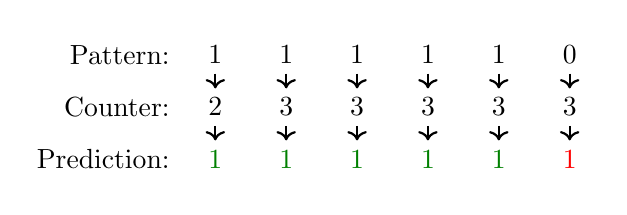
\begin{tikzpicture}[baseline=(current bounding box.center),every node/.style={anchor=base}]
    % Table for alignment
    \matrix[matrix of nodes,nodes={minimum width=0.5cm,anchor=center},column sep=0.4cm,row sep=0.2cm,ampersand replacement=\&] (m) {
        1 \& 1 \& 1 \& 1 \& 1 \& 0 \\
        2 \& 3 \& 3 \& 3 \& 3 \& 3 \\
        \textcolor{mygreen}{1} \& \textcolor{mygreen}{1} \& \textcolor{mygreen}{1} \& \textcolor{mygreen}{1} \& \textcolor{mygreen}{1} \& \textcolor{red}{1} \\
    };
    % Arrows from pattern to counter
    \foreach \i in {1,...,6} {
        \draw[->,thick] (m-1-\i.south) -- (m-2-\i.north);
        \draw[->,thick] (m-2-\i.south) -- (m-3-\i.north);
    }
    % Labels
    \node[left=0.2cm of m-1-1,align=right] {Pattern:};
    \node[left=0.2cm of m-2-1,align=right] {Counter:};
    \node[left=0.2cm of m-3-1,align=right] {Prediction:};
\end{tikzpicture}

\end{column}

\begin{column}{0.38\textwidth}
\vspace{1cm}
\begin{tcolorbox}[
    colback=lightblue!10,
    colframe=myblue,
    boxrule=1pt,
    arc=2mm,
    left=3mm,
    right=3mm,
    top=3mm,
    bottom=3mm,
    fontupper=\footnotesize\ttfamily
]
\textbf{\normalfont\small Code:}

\vspace{0.2cm}
int n = 6;

\vspace{0.2cm}
Loop: \hspace{0.3cm} ....

\vspace{0.2cm}
br1: if (n\%2) \{ ... \}

\vspace{0.2cm}
br2: if ((n+1)\%2) \{ ... \}

\vspace{0.3cm}
\hspace{0.5cm} n{-}{-};

\vspace{0.2cm}
br3: JNZ n, Loop
\end{tcolorbox}
\end{column}
\end{columns}

\end{frame}

% Section title - Conditional Branch Direction Prediction
\begin{frame}
\begin{center}
\vspace{2cm}
{\Huge\textcolor{myblue}{\textbf{Conditional Branch}}}

\vspace{0.3cm}

{\Huge\textcolor{myblue}{\textbf{Direction Prediction}}}
\end{center}
\end{frame}

% One-Bit Predictor
\begin{frame}
\frametitle{One-Bit Predictor}
\label{frame:one_bit_predictor}

\begin{center}
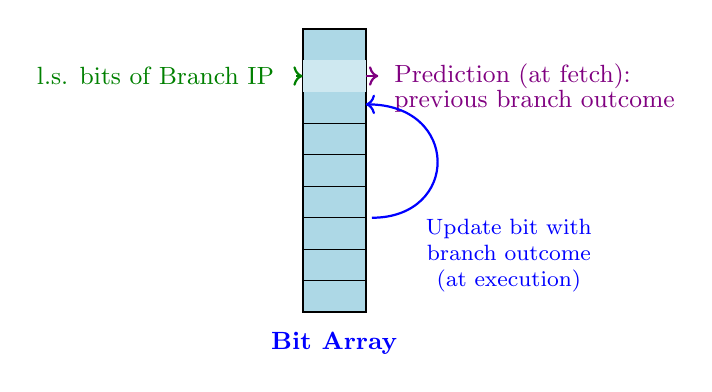
\begin{tikzpicture}[scale=0.8]
    % Draw the bit array
    \fill[lightblue] (0,0) rectangle (1,4.5);
    \draw[thick] (0,0) rectangle (1,4.5);

    % Draw array divisions
    \foreach \y in {0.5,1,1.5,2,2.5,3,3.5,4} {
        \draw (0,\y) -- (1,\y);
    }

    % Highlight one cell
    \fill[lightblue!60] (0,3.5) rectangle (1,4);

    % Labels and arrows
    \node[mygreen,anchor=east,font=\small] at (-0.3,3.75) {l.s. bits of Branch IP};
    \draw[->,thick,mygreen] (-0.1,3.75) -- (0,3.75);

    \node[mypurple,anchor=west,font=\small] at (1.3,3.75) {Prediction (at fetch):};
    \node[mypurple,anchor=west,font=\small] at (1.3,3.35) {previous branch outcome};
    \draw[->,thick,mypurple] (1,3.75) -- (1.2,3.75);

    % Curved arrow for update
    \draw[->,thick,myblue] (1.1,1.5) .. controls (2.5,1.5) and (2.5,3.3) .. (1,3.3);
    \node[myblue,align=center,anchor=west,font=\footnotesize] at (1.8,0.9) {Update bit with\\branch outcome\\(at execution)};

    % Bit Array label
    \node[myblue,font=\small\bfseries] at (0.5,-0.5) {Bit Array};
\end{tikzpicture}
\end{center}

\vspace{0.3cm}

\begin{itemize}
    \item \textbf{Problem: 1-bit predictor has a double mistake in loops}
\end{itemize}

\vspace{0.1cm}

{\footnotesize
\begin{tabular}{@{}ll@{}}
Branch Outcome & \texttt{0 0 0 0 0 1 0 0 0 0 0 1 0 0 0 0 0 1} \\
Prediction & \texttt{?~0 0 0 0 \textcolor{red}{0 1} 0 0 0 0 \textcolor{red}{0 1} 0 0 0 0 0} \\
\end{tabular}
}

\end{frame}

% 2-Level Branch Prediction
\begin{frame}
\frametitle{2-Level Branch Prediction}
\label{frame:2level_prediction}

\begin{itemize}
    \item \textbf{Save branch direction history in a Branch History Register}
    \begin{itemize}
        \item A shift-register that saves the last $n$ outcomes of the branch
        \item History points to an array of $2^n$ bits
        \item Bit pointed by a history specifies the predicted branch direction following that history
    \end{itemize}
\end{itemize}

\vspace{0.3cm}

\begin{itemize}
    \item \textbf{Example: predicting the pattern 0001 0001 0001 ...}
    \begin{itemize}
        \item History length $n=3$
    \end{itemize}
\end{itemize}

\vspace{0.2cm}

\begin{center}
% TODO: Add 2-level prediction diagram
\textcolor{red}{[PLACEHOLDER: 2-level predictor diagram showing BHR and counter array]}
\end{center}

\begin{center}
{\footnotesize
\texttt{0 0 0 | 1 0 0 0 1 0 0 0 1 ...}

\vspace{0.2cm}

\textbf{Predict at Fetch} \hspace{2cm} \textbf{Update at EXE}
}
\end{center}

\end{frame}

% Shortest History To Predict a Pattern
\begin{frame}
\frametitle{Shortest History To Predict a Pattern}
\label{frame:shortest_history}

\begin{itemize}
    \item \textbf{What is the shortest history needed to perfectly predict the pattern 10011 10011 ... in steady state?}
\end{itemize}

\vspace{0.3cm}

\begin{itemize}
    \item \textbf{A history of length 3 predicts correctly:}
    \begin{itemize}
        \item \colorbox{lightblue!30}{100}11 10011 \hspace{0.3cm} 100 $\Rightarrow$ 1
        \item 1\colorbox{lightblue!30}{001}1 10011 \hspace{0.3cm} 001 $\Rightarrow$ 1
        \item 10\colorbox{lightblue!30}{011} 10011 \hspace{0.3cm} 011 $\Rightarrow$ 1
        \item 100\colorbox{lightblue!30}{11 1}0011 \hspace{0.3cm} 111 $\Rightarrow$ 0
        \item 10011 \colorbox{lightblue!30}{1 10}011 \hspace{0.3cm} 110 $\Rightarrow$ 0
    \end{itemize}
    \item Either no sub-pattern appears more than once, or whenever the sub-pattern appears it points to the same value
\end{itemize}

\vspace{0.3cm}

\begin{itemize}
    \item \textbf{A history of length 2 is wrong twice per iteration}
    \begin{itemize}
        \item \colorbox{lightblue!30}{10}011 10011 \hspace{0.3cm} 10 $\Rightarrow$ 0
        \item 1\colorbox{lightblue!30}{00}11 10011 \hspace{0.3cm} 00 $\Rightarrow$ 1
        \item 10\colorbox{lightblue!30}{01}1 10011 \hspace{0.3cm} 01 $\Rightarrow$ 1
        \item 100\colorbox{lightblue!30}{11} 10011 \hspace{0.3cm} 11 $\Rightarrow$ \textcolor{red}{1}
        \item 10011 \colorbox{lightblue!30}{1 1}0011 \hspace{0.3cm} 11 $\Rightarrow$ \textcolor{red}{0}
    \end{itemize}
    \item A sub-pattern appears more than once, and it points to different values
\end{itemize}

\end{frame}

% Local History Predictor
\begin{frame}
\frametitle{Local History Predictor}
\label{frame:local_history}

\begin{itemize}
    \item \textbf{Use 2-bit saturating counters instead of 1 bit to record outcome}
    \begin{itemize}
        \item Avoid a double mistake in case two history sub-patterns point to the same value, or in case of a pattern glitch
        \item Example: 00001 00001 00001 01001 00001 00001
    \end{itemize}
\end{itemize}

\vspace{0.3cm}

\begin{center}
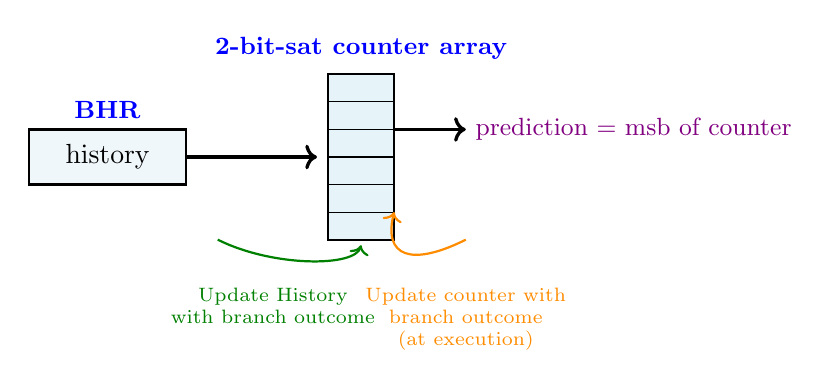
\begin{tikzpicture}[scale=0.7]
    % BHR
    \node[draw,thick,fill=lightblue!20,minimum width=2cm,minimum height=0.7cm] (bhr) at (0,0) {history};
    \node[anchor=south,font=\small\bfseries,myblue] at (bhr.north) {BHR};

    % Counter array
    \fill[lightblue!30] (4,-1.5) rectangle (5.2,1.5);
    \draw[thick] (4,-1.5) rectangle (5.2,1.5);
    \foreach \y in {-1,-0.5,0,0.5,1} {
        \draw (4,\y) -- (5.2,\y);
    }
    \node[anchor=south,font=\small\bfseries,myblue] at (4.6,1.6) {2-bit-sat counter array};

    % Arrows
    \draw[->,very thick] (bhr.east) -- (3.8,0);
    \draw[->,very thick] (5.2,0.5) -- (6.5,0.5);
    \node[anchor=west,font=\small,mypurple] at (6.5,0.5) {prediction = msb of counter};

    % Update arrows
    \draw[->,thick,mygreen] (2,-1.5) .. controls (3,-2) and (4.5,-2) .. (4.6,-1.6);
    \node[anchor=north,font=\scriptsize,mygreen,align=center] at (3,-2.2) {Update History\\with branch outcome};

    \draw[->,thick,myorange] (6.5,-1.5) .. controls (5.5,-2) and (5,-1.8) .. (5.2,-1);
    \node[anchor=north,font=\scriptsize,myorange,align=center] at (6.5,-2.2) {Update counter with\\branch outcome\\(at execution)};
\end{tikzpicture}
\end{center}

\vspace{0.3cm}

\begin{itemize}
    \item \textbf{The longer the history}
    \begin{itemize}
        \item Warm-Up is longer
        \item Counter array becomes very big (and sparse)
    \end{itemize}
\end{itemize}

\end{frame}

% Speculative History Updates - slide 1
\begin{frame}
\frametitle{Speculative History Updates}
\label{frame:speculative_history_1}

\begin{itemize}
    \item \textbf{Deep pipeline $\Rightarrow$ many cycles between fetch and branch resolution}
    \begin{itemize}
        \item If history is updated only at resolution (branch execute)
        \begin{itemize}
            \item Future occurrences of the same branch may be fetched before history is updated, and predicted with a stale history
        \end{itemize}
        \item Update history speculatively according to prediction
    \end{itemize}
\end{itemize}

\vspace{0.3cm}

\begin{center}
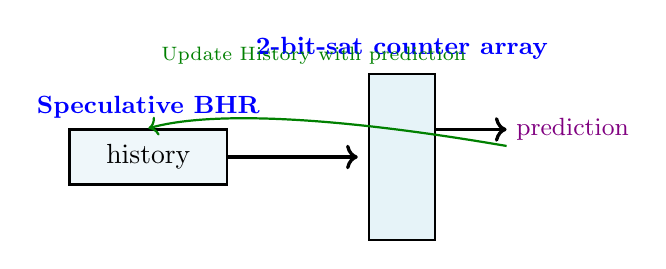
\begin{tikzpicture}[scale=0.7]
    % Speculative BHR
    \node[draw,thick,fill=lightblue!20,minimum width=2cm,minimum height=0.7cm] (sbhr) at (0,0) {history};
    \node[anchor=south,font=\small\bfseries,myblue] at (sbhr.north) {Speculative BHR};

    % Counter array
    \fill[lightblue!30] (4,-1.5) rectangle (5.2,1.5);
    \draw[thick] (4,-1.5) rectangle (5.2,1.5);
    \node[anchor=south,font=\small\bfseries,myblue] at (4.6,1.6) {2-bit-sat counter array};

    % Arrows
    \draw[->,very thick] (sbhr.east) -- (3.8,0);
    \draw[->,very thick] (5.2,0.5) -- (6.5,0.5);
    \node[anchor=west,font=\small,mypurple] at (6.5,0.5) {prediction};

    % Update with prediction
    \draw[->,thick,mygreen] (6.5,0.2) .. controls (3,0.8) and (1,0.8) .. (sbhr.north);
    \node[anchor=south,font=\scriptsize,mygreen,align=center] at (3,1.5) {Update History with prediction};
\end{tikzpicture}
\end{center}

\vspace{0.3cm}

\begin{itemize}
    \item \textbf{As long as the prediction of previous branches is correct, the history used for predicting the next branch is correct as well}
\end{itemize}

\end{frame}

% Speculative History Updates - slide 2
\begin{frame}
\frametitle{Speculative History Updates}
\label{frame:speculative_history_2}

\begin{itemize}
    \item \textbf{If a branch is mispredicted}
    \begin{itemize}
        \item History continues to be updated until the bad branch gets to execution
        \item Branches following it use a wrong history for their prediction
        \begin{itemize}
            \item But this does not matter, as they will be anyhow flushed
        \end{itemize}
        \item Need to recover the branch history to its value before the bad branch
        \begin{itemize}
            \item Maintain a non-speculative copy of the history, updated at execute
            \item In case of misprediction, copy non-speculative history into speculative history
        \end{itemize}
    \end{itemize}
\end{itemize}

\vspace{0.2cm}

\begin{center}
% TODO: Add dual BHR diagram
\textcolor{red}{[PLACEHOLDER: Diagram showing Speculative BHR and BHR with recovery mechanism]}
\end{center}

\end{frame}

% Speculative History Updates - slide 3
\begin{frame}
\frametitle{Speculative History Updates}
\label{frame:speculative_history_3}

\begin{itemize}
    \item \textbf{The counter array is not updated speculatively}
    \begin{itemize}
        \item Prediction can change only on a misprediction
        \begin{itemize}
            \item state $01\rightarrow10$ or $10\rightarrow01$
        \end{itemize}
        \item The counter array is too big to be recovered following misprediction
        \begin{itemize}
            \item Too expensive to maintain both speculative and non-speculative copies of the counter array
        \end{itemize}
    \end{itemize}
\end{itemize}

\end{frame}

% Local Predictor: private counter arrays
\begin{frame}
\frametitle{Local Predictor: private counter arrays}
\label{frame:local_private}

\textbf{Holding BHRs and counter arrays for many branches:}

\vspace{0.3cm}

\begin{center}
% TODO: Add history cache with private arrays diagram
\textcolor{red}{[PLACEHOLDER: History Cache with private counter arrays diagram]}
\end{center}

\vspace{0.3cm}

Predictor size: \#BHRs $\times$ (tag\_size + history\_size + 2 $\times$ $2^{\text{history\_size}}$)

\vspace{0.2cm}

Example: \#BHRs = 1024; tag\_size=8; history\_size=6 $\Rightarrow$

size=1024 $\times$ (8 + 6 + 2$\times$$2^6$) = 142Kbit

\end{frame}

% Local Predictor: shared counter arrays
\begin{frame}
\frametitle{Local Predictor: shared counter arrays}
\label{frame:local_shared}

\begin{itemize}
    \item \textbf{Using a single counter array shared by all BHR's}
    \begin{itemize}
        \item All BHR's index the same array
        \item Branches with similar patterns interfere with each other
        \begin{itemize}
            \item Interference can be either constructive or destructive
        \end{itemize}
    \end{itemize}
\end{itemize}

\vspace{0.3cm}

\begin{center}
% TODO: Add shared counter array diagram
\textcolor{red}{[PLACEHOLDER: History Cache with shared counter array diagram]}
\end{center}

\vspace{0.3cm}

Predictor size: \#BHRs $\times$ (tag\_size + history\_size) + 2 $\times$ $2^{\text{history\_size}}$

Example: \#BHRs = 1024; tag\_size=8; history\_size=6 $\Rightarrow$ size=1024 $\times$ (8 + 6) + 2$\times$$2^6$ = 14.1Kbit

\end{frame}

% Local Predictor: Lselect
\begin{frame}
\frametitle{Local Predictor: \textit{Lselect}}
\label{frame:lselect}

\begin{itemize}
    \item \textbf{\textit{Lselect} reduces inter-branch-interference in the counter array}
    \begin{itemize}
        \item The counter array index is a concatenation of the jump history and $m$ l.s.bits of the jump IP
        \item Counter array size becomes $2^m$ times bigger
        \item All Branches with the same $m$ IP l.s.bits interfere with each other
    \end{itemize}
\end{itemize}

\vspace{0.3cm}

\begin{center}
% TODO: Add Lselect diagram
\textcolor{red}{[PLACEHOLDER: Lselect predictor diagram with IP concatenation]}
\end{center}

\vspace{0.3cm}

Predictor size: \#BHRs $\times$ (tag\_size + history\_size) + 2 $\times$ $2^{\text{history\_size} + m}$

\end{frame}

% Local Predictor: Lshare
\begin{frame}
\frametitle{Local Predictor: \textit{Lshare}}
\label{frame:lshare}

\textbf{\textit{Lshare} reduces inter-branch-interference in the counter array:}

maps common patterns in different branches to different counters

\vspace{0.3cm}

\begin{center}
% TODO: Add Lshare diagram with XOR
\textcolor{red}{[PLACEHOLDER: Lshare predictor diagram with XOR hashing]}
\end{center}

\vspace{0.3cm}

Predictor size: \#BHRs $\times$ (tag\_size + history\_size) + 2 $\times$ $2^{\text{history\_size}}$

\end{frame}

% Global Predictor
\begin{frame}
\frametitle{Global Predictor}
\label{frame:global_predictor}

\begin{itemize}
    \item \textbf{The behavior of some branches is highly correlated}
\end{itemize}

\vspace{0.2cm}

\begin{center}
\texttt{if (x < 1) ...}

\texttt{if (x > 1) ...}
\end{center}

\vspace{0.3cm}

\begin{itemize}
    \item \textbf{Using a single Global History Register (\textit{GHR}) for all branches}
    \begin{itemize}
        \item The prediction of the 2$^{nd}$ \textit{if} is influenced by the direction of the 1$^{st}$ \textit{if}
    \end{itemize}
\end{itemize}

\vspace{0.3cm}

\begin{center}
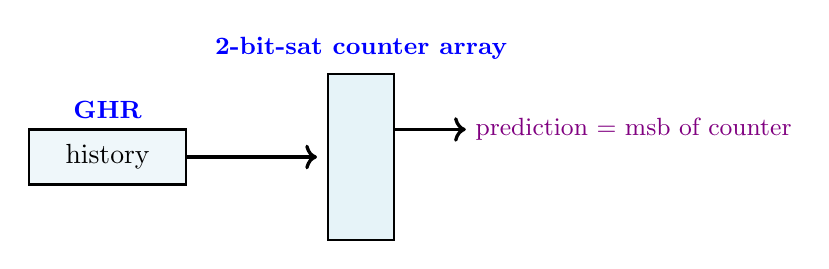
\begin{tikzpicture}[scale=0.7]
    % GHR
    \node[draw,thick,fill=lightblue!20,minimum width=2cm,minimum height=0.7cm] (ghr) at (0,0) {history};
    \node[anchor=south,font=\small\bfseries,myblue] at (ghr.north) {GHR};

    % Counter array
    \fill[lightblue!30] (4,-1.5) rectangle (5.2,1.5);
    \draw[thick] (4,-1.5) rectangle (5.2,1.5);
    \node[anchor=south,font=\small\bfseries,myblue] at (4.6,1.6) {2-bit-sat counter array};

    % Arrows
    \draw[->,very thick] (ghr.east) -- (3.8,0);
    \draw[->,very thick] (5.2,0.5) -- (6.5,0.5);
    \node[anchor=west,font=\small,mypurple] at (6.5,0.5) {prediction = msb of counter};
\end{tikzpicture}
\end{center}

\vspace{0.3cm}

\begin{itemize}
    \item \textbf{History interference between non-correlated might hurt prediction}
    \item \textbf{With only a single history, can afford a long history}
    \begin{itemize}
        \item The predictor size: history\_size + 2$\times$$2^{\text{history\_size}}$
    \end{itemize}
\end{itemize}

\end{frame}

% Global Predictor: Gshare
\begin{frame}
\frametitle{Global Predictor: \textit{Gshare}}
\label{frame:gshare}

\begin{itemize}
    \item \textbf{\textit{Gshare} combines global history information with the branch IP}
\end{itemize}

\vspace{0.3cm}

\begin{center}
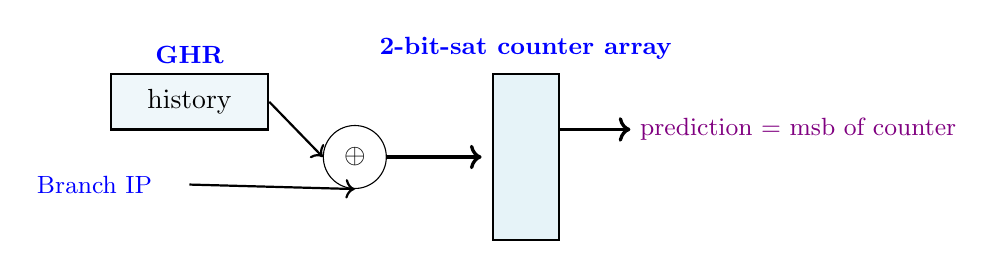
\begin{tikzpicture}[scale=0.7]
    % GHR
    \node[draw,thick,fill=lightblue!20,minimum width=2cm,minimum height=0.7cm] (ghr) at (0,1) {history};
    \node[anchor=south,font=\small\bfseries,myblue] at (ghr.north) {GHR};

    % Branch IP
    \node[anchor=east,font=\small,myblue] at (-0.5,-0.5) {Branch IP};

    % XOR
    \node[draw,circle,minimum size=0.8cm] (xor) at (3,0) {$\oplus$};

    % Counter array
    \fill[lightblue!30] (5.5,-1.5) rectangle (6.7,1.5);
    \draw[thick] (5.5,-1.5) rectangle (6.7,1.5);
    \node[anchor=south,font=\small\bfseries,myblue] at (6.1,1.6) {2-bit-sat counter array};

    % Arrows
    \draw[->,thick] (ghr.east) -- (xor.west);
    \draw[->,thick] (0,-0.5) -- (xor.south);
    \draw[->,very thick] (xor.east) -- (5.3,0);
    \draw[->,very thick] (6.7,0.5) -- (8,0.5);
    \node[anchor=west,font=\small,mypurple] at (8,0.5) {prediction = msb of counter};
\end{tikzpicture}
\end{center}

\vspace{0.3cm}

\begin{itemize}
    \item \textbf{The counter accessed is a function of the global history and of the specific branch being predicted / updated:}
    \begin{itemize}
        \item Following this history, for this specific branch, the branch is taken/NT
    \end{itemize}
    \item \textbf{This turns to be extremely accurate and space-efficient}
\end{itemize}

\end{frame}

% Why Gshare Works So Well
\begin{frame}
\frametitle{Why \textit{Gshare} Works So Well}
\label{frame:why_gshare}

\begin{itemize}
    \item \textbf{Updating a single history with all branches' outcomes might look like a mess, but ...}
\end{itemize}

\vspace{0.3cm}

\begin{itemize}
    \item \textbf{The numbers of branches active in the program at a given moment is usually small}
    \begin{itemize}
        \item E.g., in case of short loop with no if statements in the loop body
        \begin{itemize}
            \item There is only one branch in the loop (the loop's branch)
            \item Gshare behaves just like local history
        \end{itemize}
    \end{itemize}
\end{itemize}

\vspace{0.3cm}

\begin{itemize}
    \item \textbf{Assume 2 branches are active simultaneously: A and B}
    \begin{itemize}
        \item Some of the bits in the GHR are for A, and some for B
        \item Due to the XOR with their IP's, A and B update different counters
    \end{itemize}
\end{itemize}

\end{frame}

% Chooser
\begin{frame}
\frametitle{Chooser}
\label{frame:chooser}

\begin{itemize}
    \item \textbf{A chooser selects between 2 predictors for each branch}
    \begin{itemize}
        \item Use the predictor that was more correct in the past
        \item The chooser array is an array of 2-bit saturating counters, indexed by the Branch IP (similar to the Bimodal array)
        \item Updated by which predictor is more correct
    \end{itemize}
\end{itemize}

\vspace{0.3cm}

\begin{center}
% TODO: Add chooser diagram
\textcolor{red}{[PLACEHOLDER: Chooser diagram showing Global, Bimodal, and Chooser array]}
\end{center}

\vspace{0.2cm}

\begin{center}
{\small
+1 if Bimodal correct and Global wrong

-1 if Bimodal wrong and Global correct
}
\end{center}

\end{frame}

% Indirect Branch Target Prediction - slide 1
\begin{frame}
\frametitle{Indirect Branch Target Prediction}
\label{frame:indirect_target_1}

\begin{itemize}
    \item \textbf{Indirect branch targets: target given in a register}
    \begin{itemize}
        \item Can have many targets: e.g., a case statement
        \item Resolved at execution $\Rightarrow$ high misprediction penalty
        \item Used in object-oriented code (C++, Java)
    \end{itemize}
\end{itemize}

\vspace{0.3cm}

\begin{itemize}
    \item \textbf{A history-based indirect branch target predictor}
    \begin{itemize}
        \item Uses the same global history used for conditional jumps
    \end{itemize}
\end{itemize}

\vspace{0.3cm}

\begin{center}
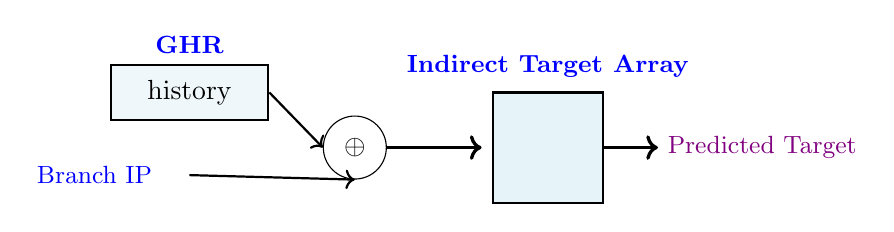
\begin{tikzpicture}[scale=0.7]
    % GHR
    \node[draw,thick,fill=lightblue!20,minimum width=2cm,minimum height=0.7cm] (ghr) at (0,1) {history};
    \node[anchor=south,font=\small\bfseries,myblue] at (ghr.north) {GHR};

    % Branch IP
    \node[anchor=east,font=\small,myblue] at (-0.5,-0.5) {Branch IP};

    % XOR
    \node[draw,circle,minimum size=0.8cm] (xor) at (3,0) {$\oplus$};

    % iTA
    \fill[lightblue!30] (5.5,-1) rectangle (7.5,1);
    \draw[thick] (5.5,-1) rectangle (7.5,1);
    \node[anchor=south,font=\small\bfseries,myblue] at (6.5,1.1) {Indirect Target Array};

    % Arrows
    \draw[->,thick] (ghr.east) -- (xor.west);
    \draw[->,thick] (0,-0.5) -- (xor.south);
    \draw[->,very thick] (xor.east) -- (5.3,0);
    \draw[->,very thick] (7.5,0) -- (8.5,0);
    \node[anchor=west,font=\small,mypurple] at (8.5,0) {Predicted Target};
\end{tikzpicture}
\end{center}

\vspace{0.3cm}

\begin{itemize}
    \item Each Jump takes multiple entries $\Rightarrow$ more expensive than TA $\Rightarrow$ should only be used for jumps with multiple targets
\end{itemize}

\end{frame}

% Indirect Branch Target Prediction - slide 2
\begin{frame}
\frametitle{Indirect Branch Target Prediction}
\label{frame:indirect_target_2}

\begin{itemize}
    \item \textbf{Initially allocate indirect branch only in the Target Array (TA)}
    \begin{itemize}
        \item Many indirect branches have only one target
    \end{itemize}
\end{itemize}

\vspace{0.2cm}

\begin{itemize}
    \item \textbf{If the TA mis-predicts for an indirect jump}
    \begin{itemize}
        \item Allocate an iTA entry with the current target
        \item Indexed by IP $\oplus$ Global History
    \end{itemize}
\end{itemize}

\vspace{0.2cm}

\begin{itemize}
    \item \textbf{Prediction from the iTA is used if}
    \begin{itemize}
        \item TA indicates an indirect jump and iTA hits
    \end{itemize}
\end{itemize}

\vspace{0.3cm}

\begin{center}
% TODO: Add TA + iTA integration diagram
\textcolor{red}{[PLACEHOLDER: Diagram showing Target Array and iTA integration with mux]}
\end{center}

\end{frame}

% Return Stack Buffer
\begin{frame}
\frametitle{Return Stack Buffer}
\label{frame:rsb}

\begin{itemize}
    \item \textbf{A return instruction is a special case of an indirect branch}
    \begin{itemize}
        \item Each times it jumps to a different target
        \item The target is determined by the location of the corresponding Call instruction
    \end{itemize}
\end{itemize}

\vspace{0.3cm}

\begin{itemize}
    \item \textbf{Maintain a small stack of targets at fetch time}
    \begin{itemize}
        \item When the Target Array predicts a Call
        \begin{itemize}
            \item Push the address of the instruction which follows the Call into the stack (this is the predicted Return address)
        \end{itemize}
        \item When the Target Array predicts a Return
        \begin{itemize}
            \item Pop a target from the stack and use it as the Return address
        \end{itemize}
    \end{itemize}
\end{itemize}

\end{frame}

% Backup section
\begin{frame}
\begin{center}
\vspace{2cm}
{\Huge\textcolor{myblue}{\textbf{Backup}}}
\end{center}
\end{frame}

% Intel 486, Pentium, Pentium II
\begin{frame}
\frametitle{Intel 486, Pentium\textsuperscript{\textregistered}, Pentium\textsuperscript{\textregistered} II}
\label{frame:intel_predictors}

\begin{itemize}
    \item \textbf{486} \hspace{1cm} Statically predict Not Taken
    \item \textbf{Pentium\textsuperscript{\textregistered}} \hspace{1cm} 2-bit saturating counters
    \item \textbf{Pentium\textsuperscript{\textregistered} II}
    \begin{itemize}
        \item 2-level, local histories, per-set counters
        \item 4-way set associative: 512 entries in 128 sets
    \end{itemize}
\end{itemize}

\vspace{0.3cm}

\begin{center}
% TODO: Add Pentium II predictor diagram
\textcolor{red}{[PLACEHOLDER: Pentium II predictor structure diagram]}
\end{center}

\end{frame}

% Alpha 264 - LG Chooser
\begin{frame}
\frametitle{Alpha 264 -- LG Chooser}
\label{frame:alpha_264}

\begin{center}
% TODO: Add Alpha 264 predictor diagram
\textcolor{red}{[PLACEHOLDER: Alpha 264 LG Chooser architecture diagram]}
\end{center}

\vspace{0.3cm}

\begin{itemize}
    \item New entry on the Local stage is allocated on a global stage mis-prediction
    \item Chooser state-machines: 2 bit each:
    \begin{itemize}
        \item one bit saves last time global correct/wrong
        \item and the other bit saves for the local correct/wrong
    \end{itemize}
    \item Chooses Local only if local was correct and global was wrong
\end{itemize}

\end{frame}


\end{document}